% Latex template: mahmoud.s.fahmy@students.kasralainy.edu.eg
% For more details: https://www.sharelatex.com/learn/Beamer

\documentclass{beamer}					% Document class
\geometry{papersize={15cm,10cm}}

\setbeamertemplate{footline}[text line]{%
  \parbox{\linewidth}{\vspace*{-8pt}\hfill\hfill\insertpagenumber}}
\setbeamertemplate{navigation symbols}{}

\usepackage[english]{babel}				% Set language
\usepackage[utf8x]{inputenc}			% Set encoding

\mode<presentation>						% Set options
{
  \usetheme{default}					% Set theme
  \usecolortheme{default} 				% Set colors
  \usefonttheme{default}  				% Set font theme
  \setbeamertemplate{caption}[numbered]	% Set caption to be numbered
}

% Uncomment this to have the outline at the beginning of each section highlighted.
%\AtBeginSection[]
%{
%  \begin{frame}{Outline}
%    \tableofcontents[currentsection]
%  \end{frame}
\usepackage{graphicx}					% For including figures
\usepackage{booktabs}					% For table rules
\usepackage{hyperref}	
\usepackage{tikz-network}				% For cross-referencing
\usepackage[absolute,overlay]{textpos}
\usepackage{bm}
\usepackage[font=small,labelfont=bf]{caption}				% For cross-referencing

\title{Probing phase transitions of DNA-protein condensates using single molecule localization microscopy}	% Presentation title
\author{Clayton W. Seitz}								% Presentation author
\date{\today}									% Today's date	

\begin{document}

% Title page
% This page includes the informations defined earlier including title, author/s, affiliation/s and the date
\begin{frame}
  \titlepage
\end{frame}


% The following is the most frequently used slide types in beamer
% The slide structure is as follows:
%
%\begin{frame}{<slide-title>}
%	<content>
%\end{frame}


\begin{frame}
\frametitle{}
\centering
\Large \textbf{\textcolor{blue}{Introduction and Approach}}
\end{frame}


\begin{frame}{Genome organization in eukaryotes}
\begin{itemize}
\item The eukaryotic genome has hierarchical structure
\item This structure is highly variable and often abberrant in disease
\end{itemize}
\begin{figure}
\includegraphics[width=13cm]{Genome.png}
\end{figure}
\textit{Finn et al., Science 365, 998 (2019)}
\end{frame}

\begin{frame}{A phase separation model for transcriptional control}
\begin{itemize}
\item Liquid-liquid phase separation (LLPS) is a major organizer of cellular biochemistry
\item Recent work highlights the importance of CTCF-dependent transcriptional condensates in determining cell fates
\end{itemize}
\begin{figure}
\includegraphics[width=13cm]{Condensates.png}
\end{figure}
\textit{Int. J. Mol. Sci. 2022, 23(14), 8039;}
\end{frame}

\begin{frame}{}
Formulate the basic research question and introduce the approach using major results from section 3
\end{frame}

\begin{frame}{Widefield/HILO fluorescence microscope}
\begin{figure}
\includegraphics[width=13cm]{Scope.png}
\end{figure}
\end{frame}


\begin{frame}
\frametitle{Direct stochastic optical reconstruction microscopy}

\begin{textblock*}{5cm}(1.5cm,1cm)
\includegraphics[width=\textwidth]{Fluorophore.png}
\end{textblock*}
  
\begin{textblock*}{6cm}(7cm,1.25cm)
\includegraphics[width=\textwidth]{Photoswitching.png}
\end{textblock*}
  
\begin{textblock*}{12cm}(1.5cm,5cm)
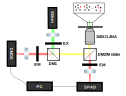
\includegraphics[width=\textwidth]{Setup.png}
\end{textblock*}
  
\end{frame}

\begin{frame}
\frametitle{Direct stochastic optical reconstruction microscopy}

\begin{figure}
\includegraphics[width=13cm]{Localization.png}
\end{figure}
  
\end{frame}

\begin{frame}{Point spread function engineering for three-dimensional imaging}
\begin{figure}
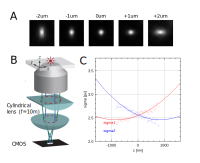
\includegraphics[width=10cm]{Astigmatism.png}
\end{figure}
\end{frame}



\begin{frame}
\frametitle{}
\centering
\Large \textbf{\textcolor{blue}{Generative models and inference for SMLM}}
\end{frame}

\begin{frame}{Statistics of sCMOS cameras}
\begin{figure}
\includegraphics[width=10cm]{Generate.png}
\end{figure}
\end{frame}


\begin{frame}{Statistics of sCMOS cameras}
\begin{itemize}
\item Each pixel of a CMOS sensor has a gain $g_{k}$ offset $o_{k}$ and readout noise variance $\sigma_{k}^{2}$
\item We measure a sum of shot noise $S_{k}$ and readout noise $\xi_{k}$
\end{itemize}
\begin{figure}
\includegraphics[width=10cm]{Kolmogorov.png}
\end{figure}
\begin{equation*}
P(H_{k}|\theta) = A\sum_{q=0}^{\infty} \frac{1}{q!}e^{-\mu_{k}}\mu_{k}^{q}\frac{1}{\sqrt{2\pi}\sigma_{k}}e^{-\frac{(H_{k}-g_{k}q-o_{k})}{2\sigma_{k}^{2}}}
\end{equation*}
\end{frame}

\begin{frame}{The model log likelihood}
Since $H_{k} = S_{k} + \xi_{k}$, we transform $H_{k}' = H_{k} - o_{k} + \sigma_{k}^{2}$, which is distributed according to 

\begin{align*}
H_{k}' \sim \mathrm{Poisson}(\mu_{k}')\;\;\;\mu_{k}' = g_{k}\mu_{k} + \sigma_{k}^{2}
\end{align*}
Since each Poisson r.v. is independent, the negative log likelihood reads
\begin{align*}
\ell(\vec{H}) &= -\log \prod_{k} \frac{e^{-\left(\mu_{k}'\right)}\left(\mu_{k}'\right)^{n_{k}}}{n_{k}!}\\
&= \sum_{k}  \log n_{k}! + \mu_{k}' - n_{k}\log\left(\mu_{k}'\right)\\
&\approx \sum_{k}  n_{k}\log n_{k} + \mu_{k}' - n_{k}\log\left(\mu_{k}'\right)
\end{align*}

\end{frame}

\begin{frame}{Localization precision for an isolated emitter}
\begin{figure}
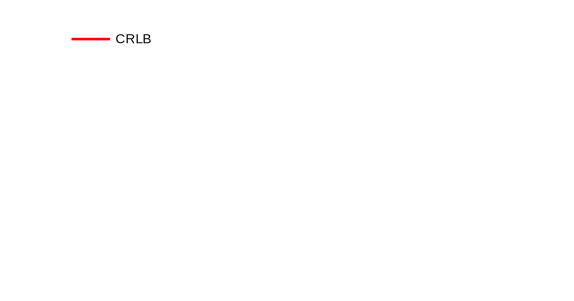
\includegraphics[width=10cm]{Errors.png}
\end{figure}
\begin{equation}
I_{ij}(\theta) = \underset{\theta}{\mathbb{E}}\left(\frac{\partial \ell}{\partial\theta_{i}}\frac{\partial\ell}{\partial\theta_{j}}\right) 
\end{equation}
\end{frame}


\begin{frame}{Estimating uncertainty with stochastic gradient langevin dynamics}
\begin{figure}
\includegraphics[width=13cm]{SGLD.png}
\end{figure}
$$dw = - \nabla L(w) dt + \epsilon \sqrt{\eta dt}, \quad \epsilon \sim \mathcal N(0, \sigma^2), \eta \propto dt$$
\end{frame}

\begin{frame}{Photoswitching dynamics are a major determinant of localization precision}
\begin{equation*}
\frac{\partial P(\omega_{i})}{\partial t} = \sum_{j}G_{ji}P(\omega_{j},t) - G_{ij}P(\omega_{i},t)
\end{equation*}
\end{frame}

\begin{frame}{A deep learning framework for localization microscopy}
Precise localization in dense regimes is intractable
\begin{figure}
\includegraphics[width=13cm]{Network.png}
\end{figure}
\end{frame}

\begin{frame}{A deep learning framework for localization microscopy}
\end{frame}

\begin{frame}{A deep learning framework for localization microscopy}
\begin{figure}
\includegraphics[width=13cm]{Jaccard.png}
\end{figure}
\end{frame}


\begin{frame}{Bayesian clustering algorithms on high density data}
Bayesian nonparametrics in general
\end{frame}

\begin{frame}{Bayesian clustering algorithms on high density data}
Bayesian nonparametrics
\end{frame}

\begin{frame}
\frametitle{}
\centering
\Large \textbf{\textcolor{blue}{Nucleosome organization in MED1-BRD4 transcriptional condensates}}
\end{frame}

\begin{frame}{Inducing GBP5 gene expression with Inteferon-$\gamma$}
\end{frame}

\begin{frame}{Colocalization of nascent GBP5 mRNA with phase separation markers}
\end{frame}

\begin{frame}{Colocalization of nascent GBP5 mRNA with phase separation markers}
\end{frame}

\begin{frame}{Costaining of H2B/BRD4/MED1 in interphase Hela cells}
\end{frame}

\begin{frame}{Cluster analysis of H2B at putative transcriptional condensates}
\end{frame}

\begin{frame}{Physical cluster analysis of H2B at putative transcriptional condensates}
\end{frame}

\end{document}